\subsection{User Trust}
    In designing assurances, which affect trust-based user behaviors, it is critical to know what drives those behaviors. Because of this some time must be spent to understand what trust is. 

    Trust is critical in interpersonal relationships, and it affects the dynamics of systems as simple as interpersonal relationships \cite{Lewicki2006-hj}, to more complicated ones such as financial markets and governments \cite{Fukuyama1995-un}. Consequently, researchers in psychology, sociology, and economics have historically sought to understand the fundamental principles of trust, each with the aim of understanding their field better \cite{Gambetta1988-pi}. Moral philosophers have also thought intently about the topic \cite{Baier1986-im}.

    Due to wide interest spanning many disciplines it is difficult, if not impossible, to write a succinct definition of trust that would appease all interested parties. Besides that, trust is actually a very broad concept that evades precise definitions at a high level. However the following definition, adapted from \cite{McKnight2004-vv}, is broad enough to avoid too much contention:

    \begin{description}
        \item [Trust:] to willingly and securely become vulnerable, or depend on, a trustee (e.g., another person, institution, or an AIA) having taken into consideration the characteristics (e.g., benevolence,  integrity,  competence)  of  the  trustee.
    \end{description}

    \subsection{Trust in AIAs?}
    \textbf{this section needs to be like two paragraphs, don't cite the entire history}
        Trust is generally understood to exist between people. Is it possible for a human to enter into a trusting relationship with an AIA? In their paper regarding important human factors that should be considered when designing autonomous machines \cite{Sheridan1984-kx} are seemingly the first to discuss the idea that trust relationships between humans and autonomous systems are important, and to suggest that humans need some assurance that the ``commands will be carried out properly''. They also mention the idea that ``there needs to be an accurate perception of [the autonomous system's] trustworthiness''. Finally they suggest that ``appropriate criteria for trust need to be studied to develop a theory of trust in supervisory control''.

        Perhaps motivated by \citeauthor{Sheridan1984-kx}\cite{Sheridan1984-kx}, a few years later \cite{Muir1987-mk}, and later in more detail \cite{Muir1994-ow}, create a psychologically based model of trust that considered the ``component expectations of trust'' of \cite{Barber1983-yc} and the dynamic evolution of trust from \cite{Rempel1985-sg}, to make a framework for studying trust in human-machine relationships.
    
        \citet{Muir1996-gt} reported the results of two experimental studies to investigate the validity of her proposed model. She claims that these were the first experiments to explicitly ask "operators to rate their trust in automated equipment", and to see if they could do so under normal operating conditions. She found that operators were able to rate their trust in the automation, and that the level of trust changed based on different performance characteristics of the automated system. In her own words: "These results suggest that operators' subjective ratings of trust and the properties of the automation which determine their trust, can be used to predict and optimize the dynamic allocation of functions in automated systems".

        That humans actually do feel trust towards machines has been experimentally confirmed several times in research using common subjective psychological questionairres. Some examples include: \citet{Muir1996-gt,Reeves1997-ad,Groom2007-bz,Mcknight2011-gv,Riley1996-qm,Bainbridge2011-pl,Kaniarasu2012-mo,Salem2015-md,Desai2012-rc, Freedy2007-sg, Wang2016-id, Inagaki1998-cl, Kaniarasu2013-ho}.

        As shown, several academic experiments have investigated the possibility of trust existing between humans and, according to the terminology of this survey, AIAs. All found that some level of trust can be formed in such relationships. \citet{Lacher2014-yc} points out that people trust an AIA at different levels. For example an operator would have different perspectives on trust based on their level of interaction with the AIA. For example the designer of an AIA would trust differently than an end user, due to the differing nature of the trust relationship from one to the other.

        \citet{Lankton2008-ct} claims, and finds some support for the idea, that trust in technology is fundamentally different from interpersonal trust between humans. They demonstrate the validity of the hypothesis by using a survey of 427 college students regarding Facebook. However, the authors point out that this study was based on a single set of survey data about facebook, and may not be unbiased or apply to other technologies. Beyond this, it is the author's opinion that the `fundamental differences' they point out are not that divergent from the human-human trust model.

        \citet{Tripp2011-cq} perform what could be considered as a follow-up experiment to \cite{Lankton2008-ct} to further investigate the variation of trust between humans and different levels of technology. They run experiments with three different levels of technology: MS Access, a recommender system, and Faceobook. They found that `human-like' trust applied more to Facebook, while `system-like' trust applied more to MS Access. They conclude that if the system is ``human enough'' then a human trust model is appropriate, but caution that it is important to check first.

        Given this research, we will take the position of presenting a human-human trust model and using it as a basis for human-AIA trust. With the understanding that the applicability of the model varies with the complexity of the AIA. For example from something in the lower-left quadrant of \ref{fig:StrongWeak} to the upper-right quadrant.

    \subsection{A Model of Human-AIA Trust}
        Returning to the main focus of this section, we now present a model of human-AIA trust, with the expectation that this model will cast insights on assurances that can be used later. It should be noted that \emph{this model} is being present as one model that can be helpful in understanding assurances, but it may not be \emph{the} perfect model. As research advances it will probably change, and the ideas of assurances will naturally change as well. \textbf{needs work}.

        This has been recently attempted in the context of human-AIA relationships \cite{Lahijanian2016-nd}, but with an overly simplistic reduction of trust. The reality is that trust is extremely complex, and so dealing with it in the setting of human-AIA relationships is going to be complex.

        In work relating to business management \citet{McKnight1998-ty} and later in \cite{McKnight2001-fa} performed what is, to my knowledge, the first multi-disciplinary survey and unification of trust literature, and condensed it into a single typology. That model is shown, with some minor adaptations, in Figure \ref{fig:UserTrust}. Notice that the three main dimensions --- Dispositional Trust, Institutional Trust, and Interpersonal Trust --- are connected in such a way as to indicate some causal relationships between them.

        \begin{figure}[htbp]
            \centering
            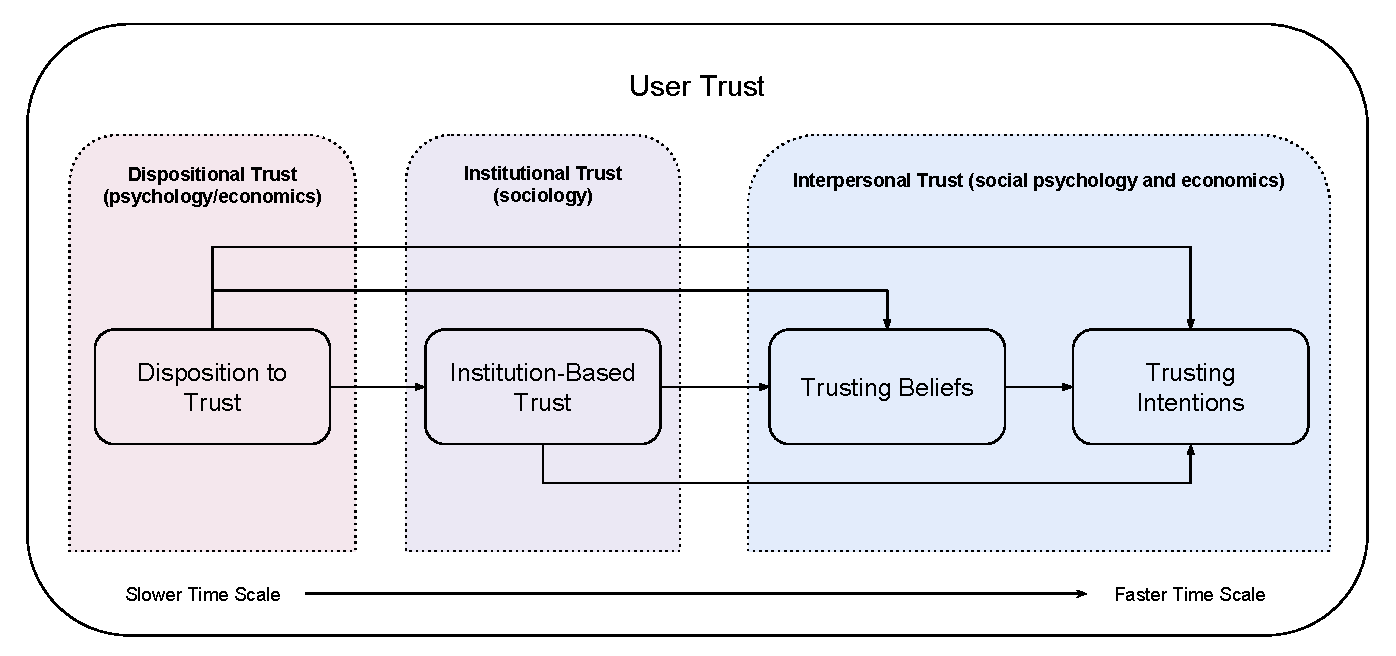
\includegraphics[width=0.9\textwidth]{Figures/UserTrust}
            \caption{Interdisciplinary trust model proposed by \citet{McKnight2001-fa}. The three main categories are delineated, and corresponding disciplines that are interested are listed within parentheses.}
            \label{fig:UserTrust}
        \end{figure}

        The categories are defined as follows:

        \begin{description}
            \item [***NOTE***:] \textbf{Perhaps provide examples in the human-AIA context to help ground the definitions}
            \item [Disposition to Trust:] The extent to which one displays a consistent tendency to be willing to depend on others in general across a broad spectrum of situations and persons
            \item [Institution-Based Trust:] One believes that favorable conditions are in place that are conducive to situational success in an endeavor or aspect of one's life
            \item [Trusting Beliefs:] One believes that the other party has one or more characteristics beneficial to oneself
            \item [Trusting Intentions:] One is willing to depend on, or intends to depend on, the other party even though one cannot control that party
        \end{description}

        Each of these main categories has components defined in Figure \ref{fig:Assurance_classes}. These components were defined through the compilation of many research studies across research disciplines, and because of this represent the most accurate notion of the components of trust available. We propose that these trust components describe the possible dimensions that constitute trust-related behaviors, and at which assurances must be targeted.

        \begin{sidewaysfigure}[htbp]
            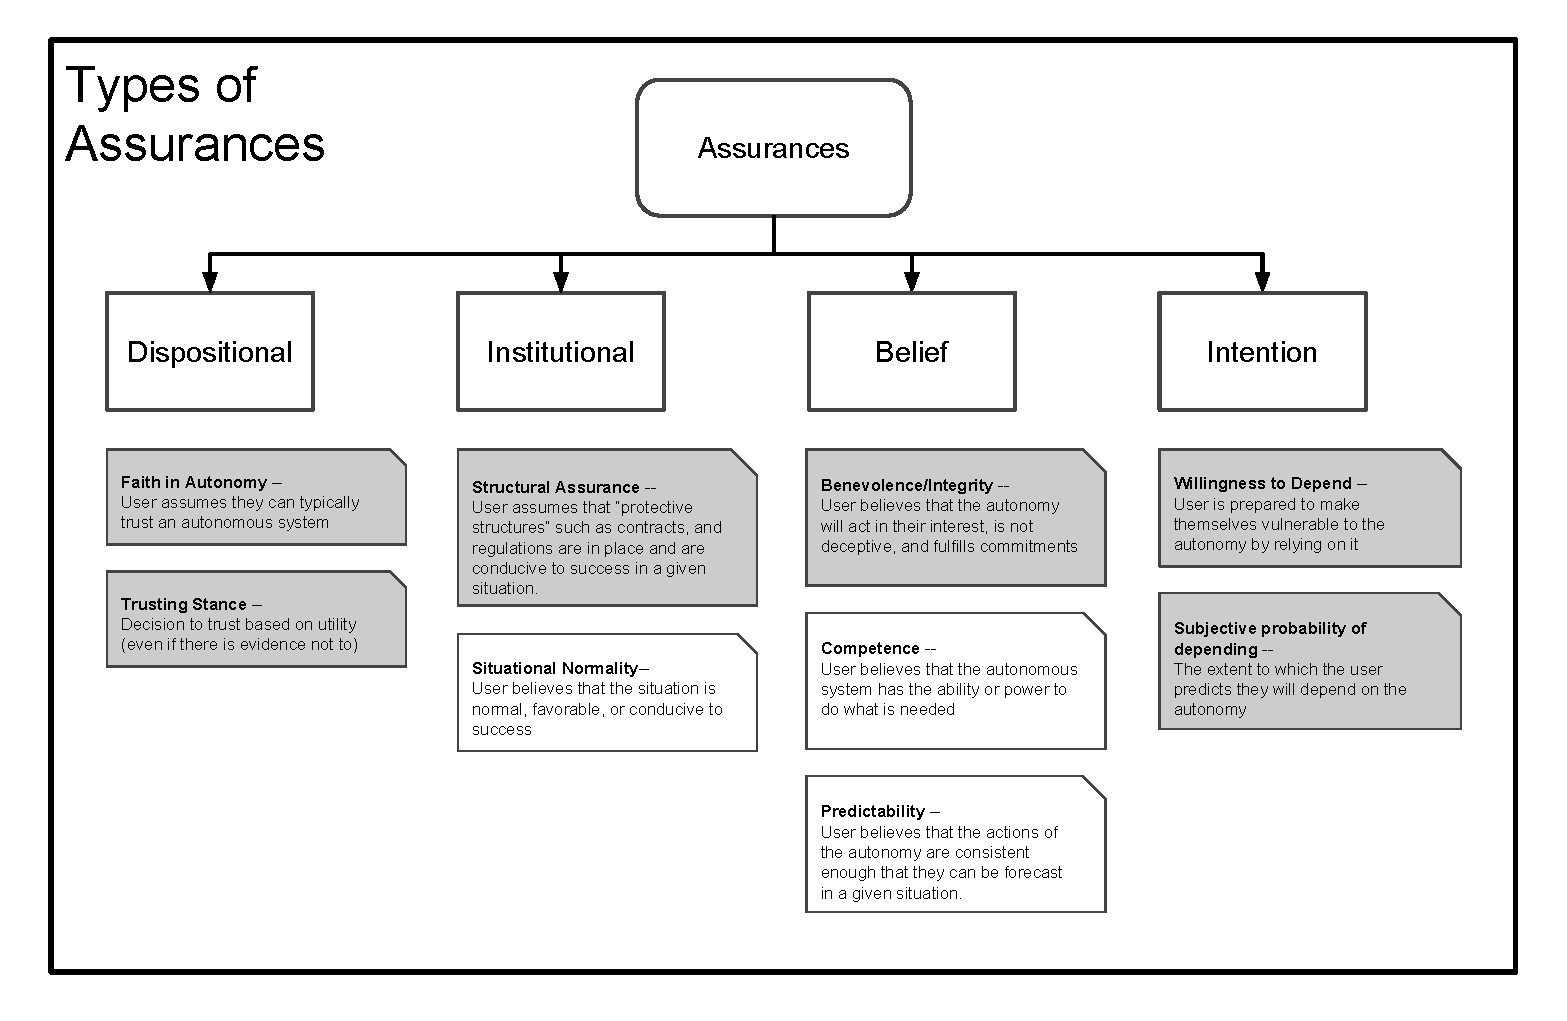
\includegraphics[width=8in]{Figures/Assurances.pdf}%
            \caption{\textbf{Diagram delineating the possible classes of assurances, and suggesting those classes that directly apply in calibration of TRBs \ldots obviously needs to be finished \ldots}}
            \label{fig:Assurance_classes}
        \end{sidewaysfigure}

    \subsection{A Note Regarding Distrust}
    \textbf{maybe move to the end of the paper, maybe a future work section?}
        For completeness it is important to mention distrust, although it will not be a that is directly addressed in this paper. As reviewed and discussed by \citet{Lewicki1998-ox}, and formalized in \cite{McKnight2001-hm,McKnight2001-gz} low trust is not the same as distrust, neither is low distrust the same as trust. \citet{McKnight2001-gz} suggest that ``the emotional intensity of distrust distinguishes it from trust''. They explain that distrust comes from emotions like: wariness, caution, and fear. Whereas, trust stems from emotions like: hope, safety, and confidence. Trust and distrust are orthogonal elements that define a person's TRB towards a trustee. \citet{Lewicki1998-ox} list several behaviors that stem from different combinations of trust and distrust; these are shown in Figure \ref{fig:distrust_table}.

        \begin{figure}[!htbp]
            \centering
            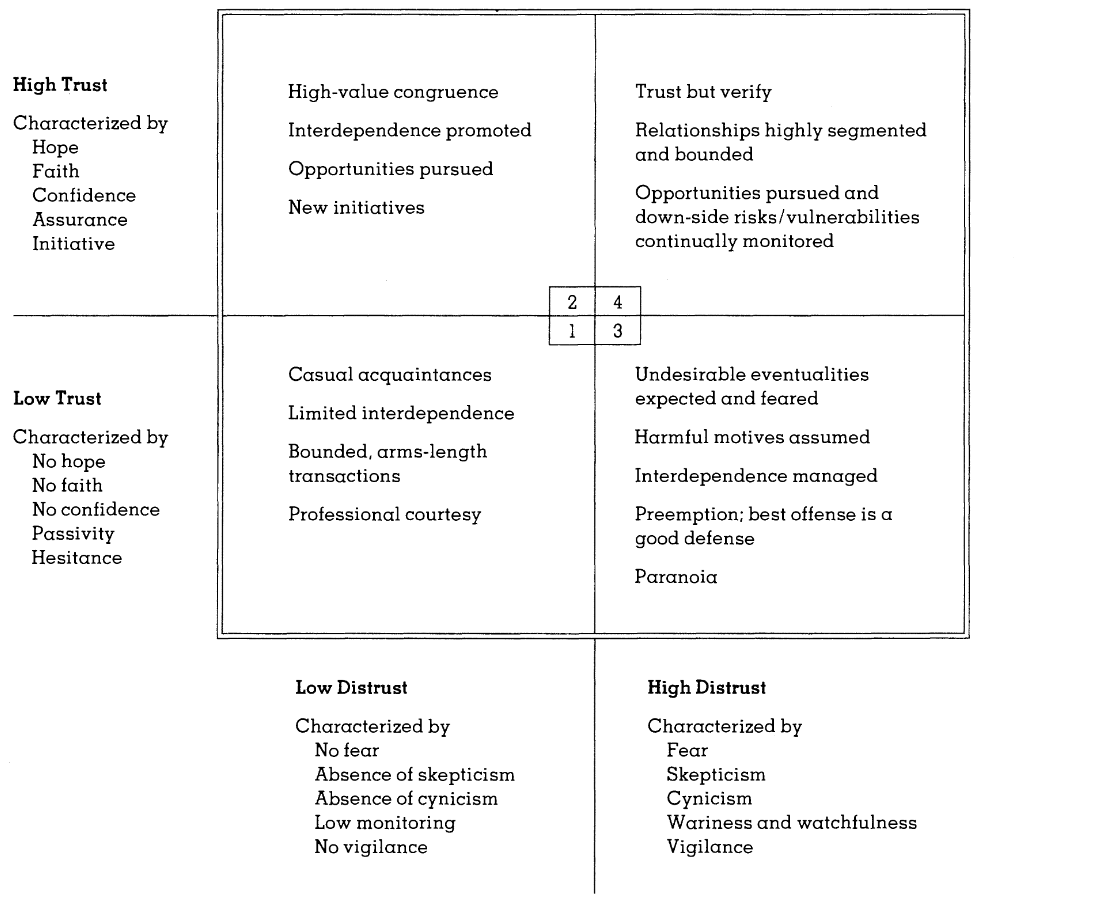
\includegraphics[width=0.6\textwidth]{Figures/distrust_table}
            \caption{Trust--Distrust table from \cite{Lewicki1998-ox}}
            \label{fig:distrust_table}
        \end{figure}

        In \citet{McKnight2001-gz} models for trust and distrust are proposed, and in later studies empirical evidence to validate some of the dimensions of both models was performed. \citet{McKnight2002-qx} is an empirical study that validates the model and quantifies the relationships between the model dimensions, and \citet{McKnight2004-vv} investigates and quantifies the relationship between dispositional distrust and web-site usage. Finally, \citet{McKnight2006-ce} revisits the position of \citet{McKnight1998-ty} and concludes that research had largely confirmed the model.

        \textbf{add a small mention of McKnight's definition that distrust is the total opposite of trust?}

        In this survey distrust will not be considered; this is in a effort to reduce the scope, which is already at risk of being too large. However, it must be made clear that any \emph{complete} treatment of trust relationships, and for our purposes, designed assurances, must consider the dimensions of distrust as well as those of trust. 
        
        Distrust has been shown to vary with perceived risk \cite{McKnight2004-vv}. This means that the implicit assumption of this paper is that risk in 1-on-1 human-AIA relationships is held constant. We claim that this is a realistic assumption for many practical applications.
